% =============================================================
%  Switchgear of the recovery — AC circuit breaker, insertion resistor
%  with bypass switch, discharge units, DC disconnect switches.
%  Figure: fig/dc_frt.pdf, the single-line of one converter station,
%  cast by Glyphwright from examples/sld/dc_frt.yaml in
%  ~/Projects/glyphwright (python -m glyphwright sld examples/sld/dc_frt.yaml).
% =============================================================
\subsection{Switchgear of the Recovery}
\label{sec:dcf-switchgear}

Figure~\ref{fig:dcf-switchgear} shows the single-line diagram of one
converter station with the switchgear a recovery sequence operates~[24],
[25]. Four devices take part:

\begin{itemize}[itemsep=0.2em]
  \item \textbf{AC circuit breaker.} Clears the fault by separating the
        diode rectifier from the AC network, and re-energises the interface
        transformer and the converter at the restart.
  \item \textbf{Insertion resistor and bypass switch.} The insertion
        resistor is in series with the network terminals of the interface
        transformer and is bypassed in normal operation. For the restart the
        bypass switch is opened before the circuit breaker closes, so the
        DC circuit is charged through the resistor and the diodes. The
        resistor limits the inrush of the diodes and, if the fault
        persists, the uncontrolled fault current. Once the charging current
        has decayed the bypass switch closes and the converter is
        deblocked.
  \item \textbf{Discharge unit.} One per pole: a fast-acting grounding
        switch in series with a damping resistor. It removes the trapped
        charge of the healthy pole after a pole-to-ground fault, and is
        closed only for that purpose. The resistance is chosen well above
        the surge impedance of the DC circuit so that the discharge does not
        launch travelling waves of its own~[24]. One station leads the
        discharge, the unit of the other being the backup~[25].
  \item \textbf{DC disconnect switches.} Slow devices that separate a
        converter station from the DC circuit for STATCOM operation. Their
        operating time is one of the two terms that set the changeover time
        of Section~\ref{sec:dcf-zones-statcom}.
\end{itemize}

\begin{figure}[!ht]
  \centering
  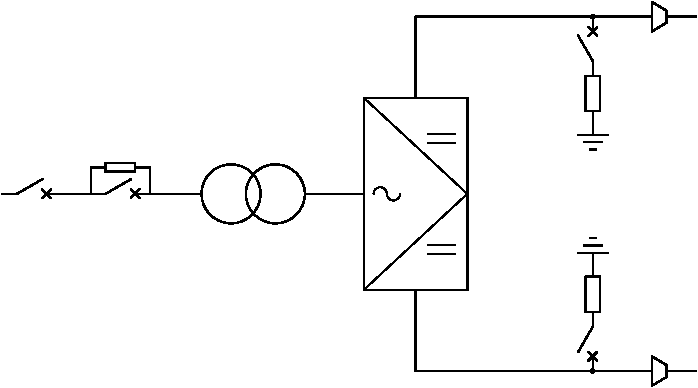
\includegraphics[width=0.85\linewidth]{dc-fault-ride-through/fig/dc_frt.pdf}
  \caption{Switchgear of one converter station taking part in the DC line
           fault recovery, after~[24]; from left: AC circuit breaker,
           insertion resistor with its bypass breaker, interface
           transformer, converter, and on each pole a discharge unit
           (grounding switch and damping resistor) and the cable sealing
           end towards the DC circuit}
  \label{fig:dcf-switchgear}
\end{figure}

\FloatBarrier
